% \slide{Características do Tráfego}{
%     O tráfego é afetado por diversos fatores.

%     \begin{itemize}
%         \item \textbf{Fatores Temporais}. Ex: Alto fluxo causado pelo horário do expediente dos trabalhadores;
%         \item \textbf{Fatores Espaciais}. Ex: Locais que podem ter mais ou menos movimento de veículos (áreas rurais, urbanas, próximas de empresas, etc);
%         \item \textbf{Fatores Aleatórios}. Ex: Eventos impossíveis de prever que podem afetar o fluxo de veículos, como acidentes automobilísticos;
%     \end{itemize}
    
%     % should we talk here that we are only gonna use temporal and spatial features or we just talk about it?
% }

%colocar referncia do artigo que demonstra como se calcula a densidade : Short-Term Traffic Prediction Using Long Short-Term Memory Neural Networks Zainab Abbas et al

\slide{Aquisição}{
    \begin{itemize}
        \item DETRAN;
        \item Série Temporal de Registro de Veículos;
        \item Avenida Hélio Prates;
        \item Maio a Junho de 2016;
        \item 8 sensores disponíveis;
        \item Não foram encontrados falhas nos dados, sem valores nulos ou falta de dados que poderiam afetar o experimento;
    \end{itemize}
}

\slide{Caracterização dos Dados}{
    \begin{table}[htbp]
        \begin{tabular}{ccccccc}
        \toprule
        \multicolumn{1}{l}{\textbf{Id Equi.}} & \multicolumn{1}{l}{\textbf{A/M/D}} & \multicolumn{1}{l}{\textbf{Hora}} & \multicolumn{1}{l}{\textbf{Faixa}} & \multicolumn{1}{l}{\textbf{km/h}} & \multicolumn{1}{l}{\textbf{km/h Max}} & \multicolumn{1}{l}{\textbf{Tam.}} \\ 
        \midrule
        RSI128 & 2016/5/1 & 00:00:09 & 1 & 20 & 60 & 0 \\
        RSI131 & 2016/5/1 & 00:00:09 & 2 & 45 & 60 & 1.1 \\
        RSI132 & 2016/5/1 & 00:00:09 & 1 & 40 & 60 & 0 \\
        RSI131 & 2016/5/1 & 00:00:10 & 1 & 35 & 60 & 0.5 \\ 
        \bottomrule
        \end{tabular}
        \caption{Colunas dos dados registrados pelos fiscalizadores eletrônicos}
    \end{table}
}

\slide{Cruzamento 1}{
    \begin{figure}[htbp]
        \centering
        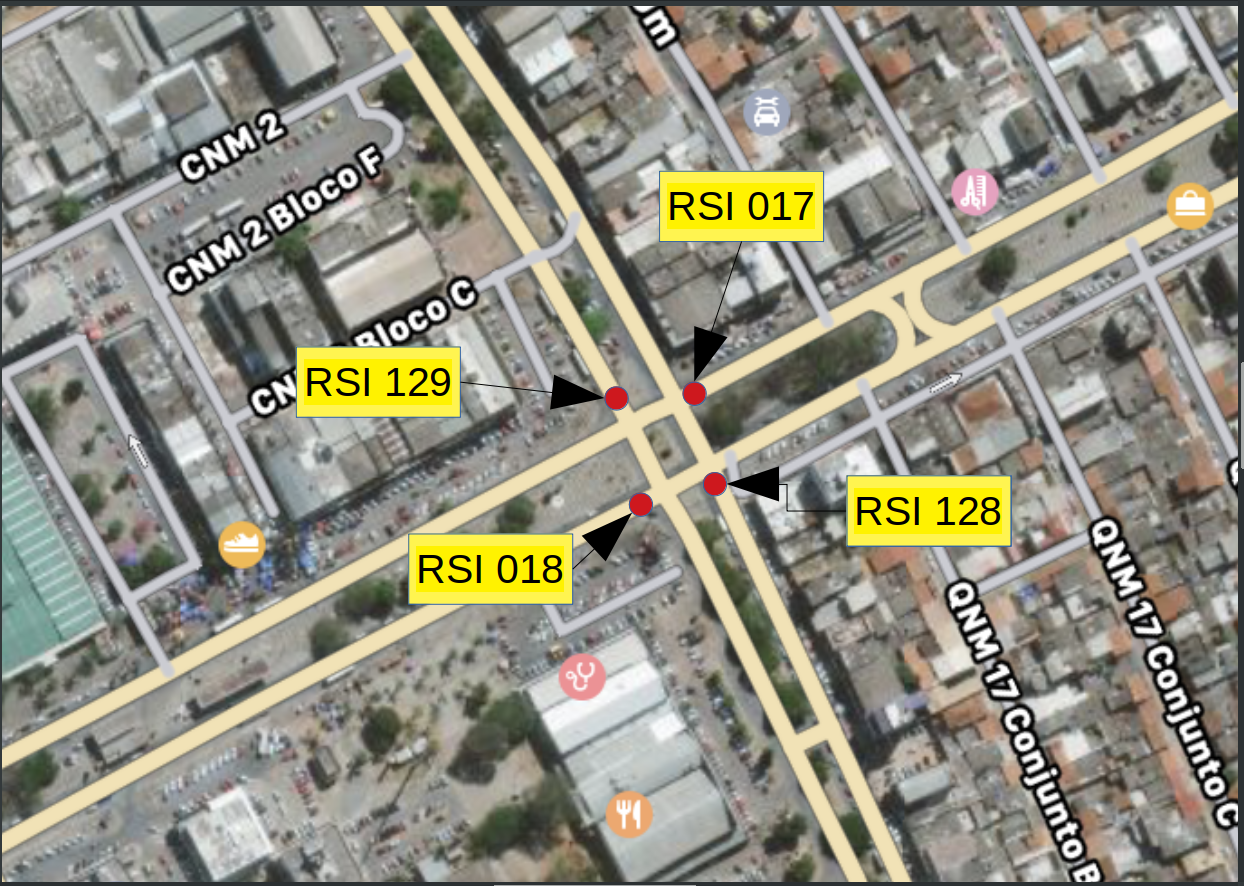
\includegraphics[scale=0.2]{monography/img/maps/crossing_1.png}
    \end{figure}
}

\slide{Cruzamento 2}{
    \begin{figure}[htbp]
        \centering
        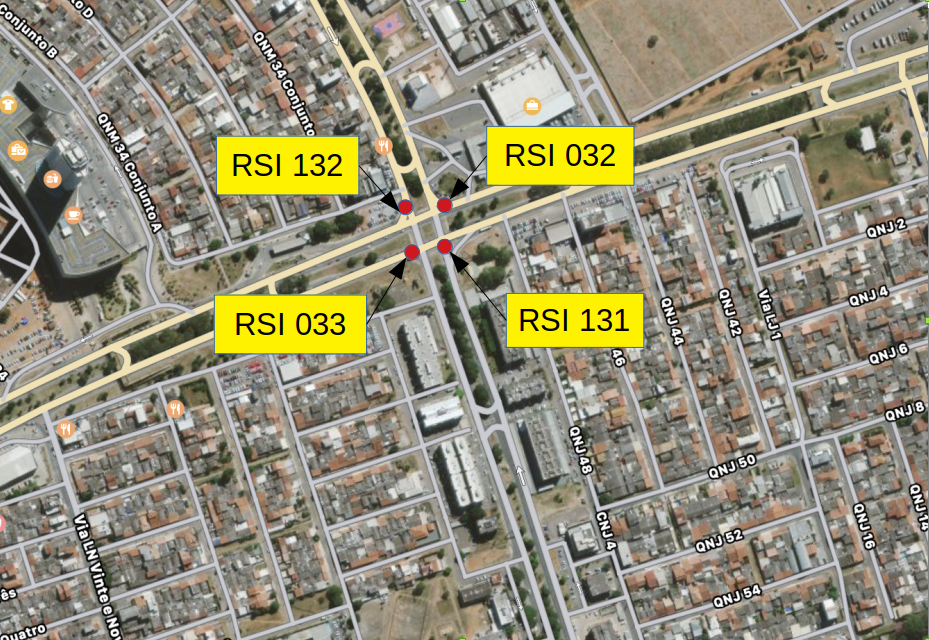
\includegraphics[scale=0.3]{monography/img/maps/crossing_2.png}
    \end{figure}
}
